\metroset{sectionpage=none}
\section{Глава 2. Разработка метода, способного оперировать действиями различного масштаба, устойчивого к шумам, и его применение для настройки оптического интерферометра 
}

\begin{frame}
    \frametitle{Структура диссертационной работы}
    \begin{itemize}
        \item \underline{Глава 1.} Обзор методов обучения с подкреплением и их применения в роботике. 
        {\color{orange}\item \underline{Глава 2.} Разработка метода, способного оперировать действиями различного масштаба, устойчивого к шумам, и его применение для настройки оптического интерферометра (вызов 1,2).}
        \item \underline{Глава 3.} Метод, который позволяет достичь сходимости к хорошему оптимуму для многозадачного агента и его применение  для управления движением шагающего робота (вызов 3).
        \item \underline{Глава 4.} Иерархический алгоритм, комбинирующий алгоритмический и нейросетевой подходы и его применение для управления агентом в среде NetHack (вызов 4).
    \end{itemize}
\end{frame}


\begin{frame}{Постановка задачи оптимизации}

$$Q(s_t,a_t) = \ex_{r_{t+1},s_{t+1}}\left[r_{t+1} + \gamma \max_{a^{\prime} \in \mathcal{A}}Q(s_{t+1},a^{\prime})\right]$$
$$\pi = \argmax_{a \in \mathcal{A}}Q(s,a)$$

Особенности:
\begin{enumerate}
    \item Произвольное начальное состояние $s_0 \in \mathcal{S}$.
    \item Оптимальная стратегия должна оперировать действиями различного масштаба $a \sim \pi^*(s): \color{red}{\min(|a|) \ll \max(|a|)}$.
    \item Высокая размерность пространства состояний $s \in \mathcal{R}^N$
    \item Перенос из симуляции на физическую установку.\\
    Обучение: \hspace{12pt}$s_{t+1} \sim p_{\mathrm{sim}}(s_t, a_t)$.\\
    Применение: $s_{t+1} \sim {\color{red}p_{\mathrm{exp}}}(s_t, a_t + {\color{red}\zeta})$.
\end{enumerate}
\end{frame}

\begin{frame}{Алгоритм 1: Подбор параметров симулятора и их рандомизация \footnotemark \footnotemark}

\vspace{-10pt}
\begin{minipage}{\linewidth}

\begin{columns}
\column{0.5\linewidth}
Train: $s_{t+1} \sim p_{\mathrm{sim}}(s_t, a_t, \theta_1, ..., \theta_n)$
Test: $s_{t+1} \sim {\color{red}p_{\mathrm{exp}}}(s_t, a_t + {\color{red}\zeta})$
\vspace{10pt}
\begin{enumerate}
    \item Подбирем средние значения параметров $\theta_1, ..., \theta_n$: $<s_{\mathrm{sim}}>$ $\sim$ $<s_{\exp}>$

    \item Зашумляем $\theta \gets [\theta_{\min}, \theta_{\max}]$ для устойчивости к шумам
\end{enumerate}

\column{0.5\linewidth}
\begin{algorithm}[H]
\KwData{
$<s_{\exp}> \sim p_{\exp}(s_t, a_t)$\\
$<s_{\mathrm{sim}}> \sim p_{\mathrm{sim}}(s_t, a_t, \theta)$
}
\KwResult{$\theta_1, ..., \theta_n$} 
$\varepsilon \gets f(<s_{sim}>, <s_{\exp}>)$\;
\While{$\varepsilon > \varepsilon_{\min}$}{
  $\theta$ = optimizer.step()\;
  $<s_{\mathrm{sim}}> \sim p_{\mathrm{sim}}(s_t, a_t, \theta)$\;
  $\varepsilon \gets f(<s_{sim}>, <s_{\exp}>)$\;
}
\end{algorithm}
Подбор значений параметров $\theta$. 
\end{columns}
\end{minipage}

%\vspace{10pt}
\begin{minipage}{\linewidth}
\fontsize{8pt}{10pt}\selectfont
    \emph{Замечание}: Если агент устойчив к шуму в наблюдениях, то шум в действиях $a_t + \zeta$ не будет влиять на стратегию агента, если он является несмещенным $\ex (a_t + \zeta) = a_t$
\end{minipage}

\setcounter{footnote}{0} 
\footnotetext[1]{Peng, X. B., Andrychowicz, M., Zaremba, W., Abbeel, P. Sim-to-Real Transfer of Robotic Control with Dynamics Randomization. ICRA, 2018.}
\footnotetext[2]{Rao, K., Harris, C., Irpan, A., Levine, S., Ibarz, J., and Khansari, M. RL-CycleGAN: Reinforcement Learning Aware Simulation-to-Real. CVPR, 2020.}

\end{frame}

\setcounter{footnote}{0} 
\begin{frame}{Алгоритм 2: Масштабирование действий\footnotemark}

\vspace{-20pt}
\begin{minipage}{\linewidth}
\begin{columns}
\column{0.5\linewidth}
\begin{align*}
& a \in \mathcal{R}^n: a_i \in [-1, 1] \\
& \text{параметр } b \gg 1\\ 
& a_i^{\prime} =
   \begin{cases}
    {\mathrm{sign}}(a_i) \cdot b^{|a_i| - 1}, |a_i| > a_{\min}
    \\
    0
  \end{cases}
\end{align*}

\column{0.5\linewidth}
\begin{figure}
    \centering
    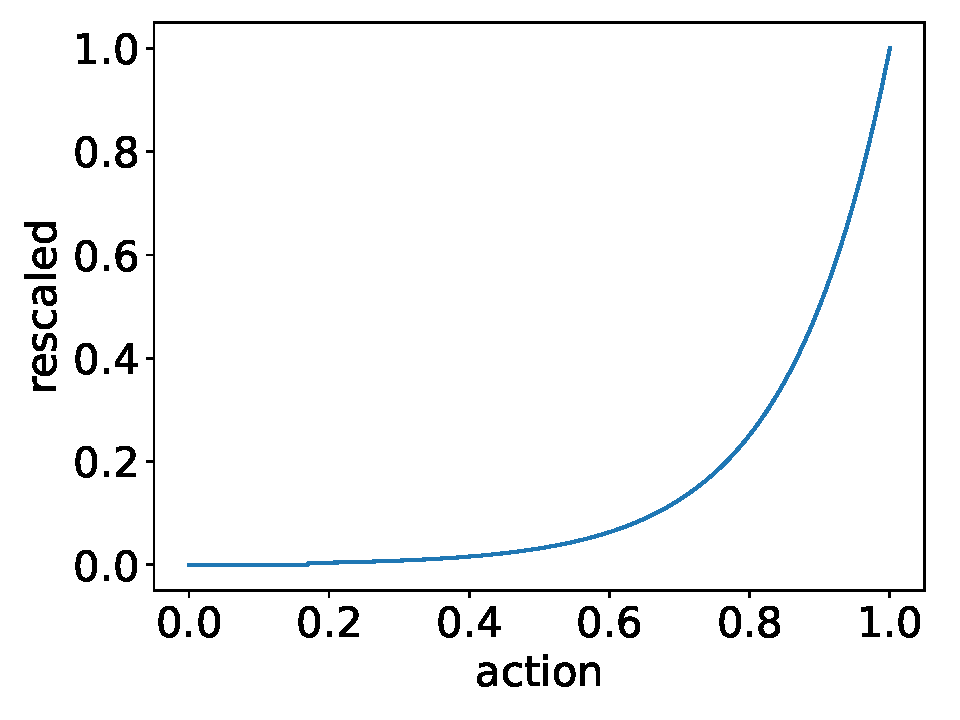
\includegraphics[width=1\linewidth]{images/rescale.pdf}
\end{figure}

\end{columns}
\end{minipage}

\vspace{-10pt}
\begin{minipage}{\linewidth}
\begin{columns}
\column{0.5\linewidth}
\centering Пример: CartPole Continous
\vspace{5pt}
    \begin{tabular}{c|c|c}
         & return & position \\ 
         \hline
         rescaled &  2756 $\pm$ 842 & -0.04 $\pm$ 0.09\\
         raw & 1692 $\pm$ 932 & 0.03 $\pm$ 0.22 
    \end{tabular}

\vspace{10pt}\hspace{-5pt} $r = -\log(|x| + 10^{-5})$  


\column{0.5\linewidth}
\begin{figure}
    \centering
    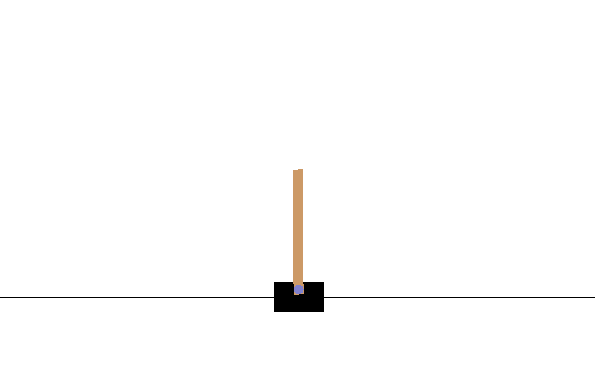
\includegraphics[width=0.8\linewidth]{Presentation/images/cartpole.png}
\end{figure}
\end{columns}
\end{minipage}

\footnotetext[1]{Dadashi, R., Hussenot, L., Vincent, D., Girgin, S., Raichuk, A., Geist, M., Pietquin, O. Continuous Control with Action Quantization from Demonstrations, ICML, 2022}

\end{frame}



\begin{frame}{Практическая задача: Настройка оптического интерферометра}
\vspace{-30pt}
\begin{figure}
  \centering
  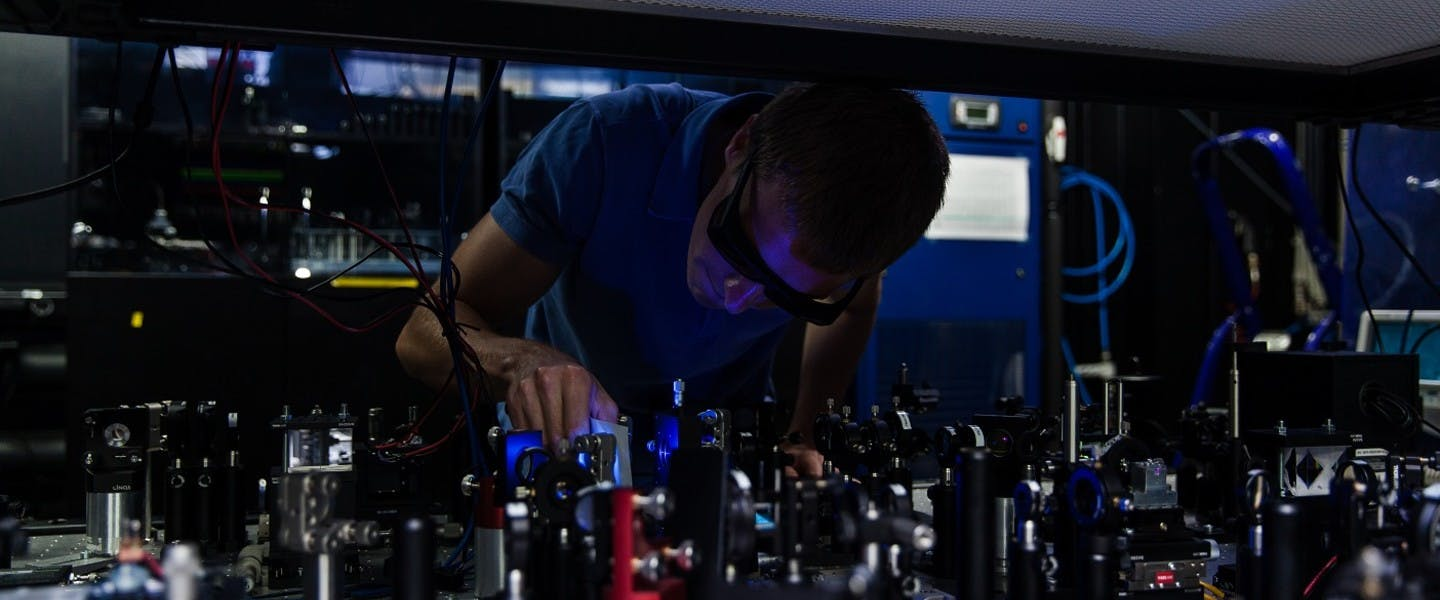
\includegraphics[width=1\linewidth]{Presentation/images/labinterf.jpg}
\end{figure}
\vspace{-10pt}

\setcounter{footnote}{0} 
Смежные задачи рассматривались в работах\footnote{Degrave, J., Felici, F., Buchli, J. et al. Magnetic control of tokamak plasmas through deep reinforcement learning. Nature, 2022.}
\footnote{Chen, IJ., Aapro, M., Kipnis, A. et al. Precise atom manipulation through deep reinforcement learning. Nat Commun, 2022.}
\end{frame}

\subsection{Постановка задачи}

\begin{frame}
\frametitle{Физические принципы работы и модель оптического интерферометра}
\begin{columns}
\column{0.5\linewidth}
  \centering
  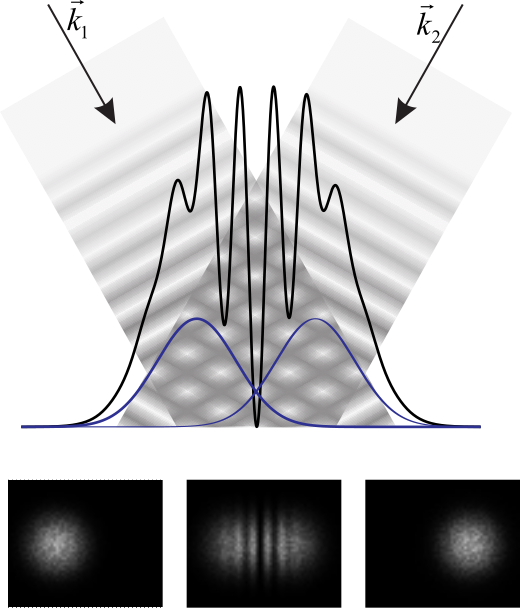
\includegraphics[width=0.9\linewidth]{images/interf_expl.png}

\column{0.5\linewidth}

\begin{align*}
& E(x,y,z)=\exp \left[-\frac{\left(x-x_{0}\right)^{2}+\left(y-y_{0}\right)^{2}}{r^{2}(z)}\right] \cdot \\
& \hspace{20pt} \exp \left[-i\left(k_{x} x+k_{y} y+k_{z} z + k\frac{x^2+y^2}{2\rho^2(z)} z\right)\right] \\
& E(x, y, z) = E_1(x, y, z) + E_2(x, y, z) \\
& I(x, y, z) = |E(x, y, z)|^2 = E(x,y,z) \cdot E^*(x,y,z) \\
& I= I_1 + I_2 + 2 \sqrt{I_1I_2}\cos(\Delta \phi)
\end{align*}

\end{columns} 
\end{frame}

\begin{frame}
\frametitle{Интерферометр Маха-Цендера}
  \centering
  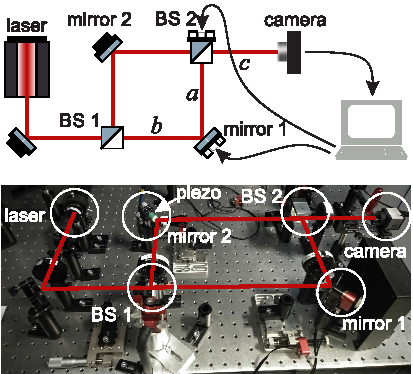
\includegraphics[width=0.8\linewidth]{scheme_with_experiment.pdf}
\end{frame}


\begin{frame}
\frametitle{Математическая модель интерферометра Маха-Цендера}
\begin{minipage}{\textwidth}
\begin{columns}
\column{0.6\linewidth}
  \centering
  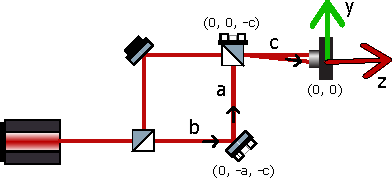
\includegraphics[width=1\linewidth]{images/MZI_matmodel.pdf}
  
\column{0.5\linewidth}
\begin{itemize}
    \item управление положением луча на камере $(x_0, y_0)$
    \item управление направлением $\vec{k}$
  \end{itemize}
\end{columns}
\end{minipage}

\vspace{20pt}

\begin{minipage}{\textwidth}
\begin{columns}
\column{0.6\linewidth}
  \centering
  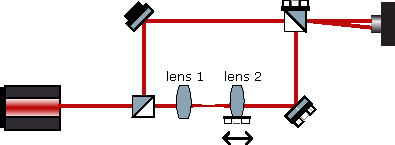
\includegraphics[width=1\linewidth]{images/MZI_expl_lenses.pdf}
  
\column{0.5\linewidth}
\begin{itemize}
    \item \textcolor{red}{управление волновым фронтом}
  \end{itemize}
\end{columns}
\end{minipage}
\end{frame}


\begin{frame}{Численная модель интерферометра Маха-Цендера}
\begin{columns}
\column{0.5\linewidth}
\centering
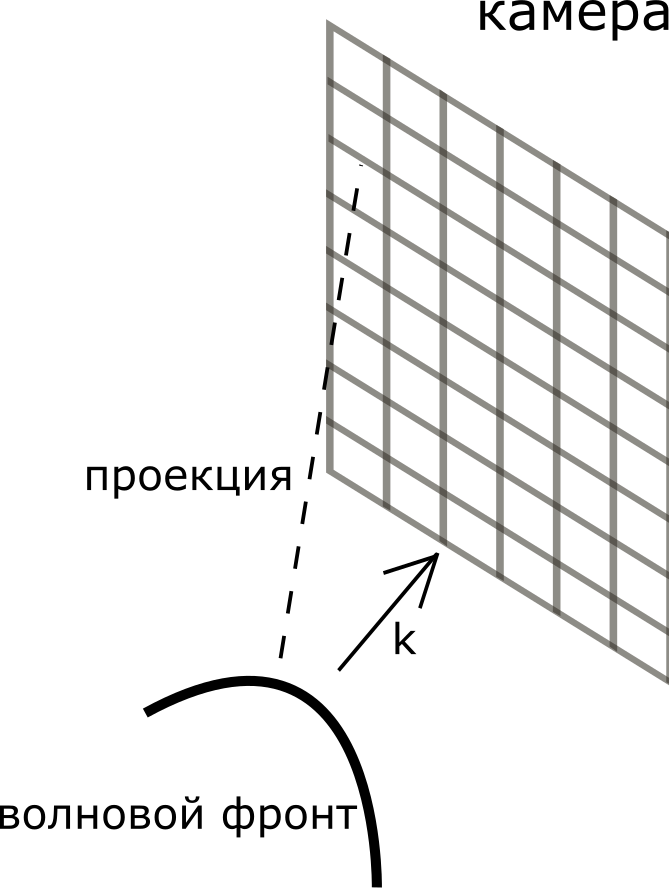
\includegraphics[width=0.8\linewidth]{images/wave_front_projection.png}
\column{0.5\linewidth}
\begin{enumerate}
    \item трассировка лучей 
    \begin{itemize}
        \item прохождение через зеркала $\vec{k}$, $(x_0, y_0)$
        \item радиус $r(z)$ и волновой фронт $\rho(z)$
    \end{itemize}
    \item вычисление интерференционной картины
    \begin{itemize}
        \item пространственное разрешение 64×64 пикселя
        \item временное разрешение 16 кадров
        \item параллельно для каждого пикселя и кадра
    \end{itemize}

    
\end{enumerate}

\end{columns}
\end{frame}



\begin{frame}
\frametitle{Интерференционная картина, полученная в эксперименте}
\begin{minipage}{\textwidth}

\begin{equation*}
\hspace{1000pt minus 1fil}
\text{Видность интерференционной картины }
    V = \frac{            
        \max_{t}(I_{\mathrm{tot}}) - \min_t(I_{\mathrm{tot}})}
        {\max_{t}(I_{\mathrm{tot}}) + \min_t(I_{\mathrm{tot}})}
\hfilneg
\end{equation*}
\end{minipage}

\begin{minipage}{\textwidth}
\begin{columns}
\column{0.7\linewidth}
\centering
    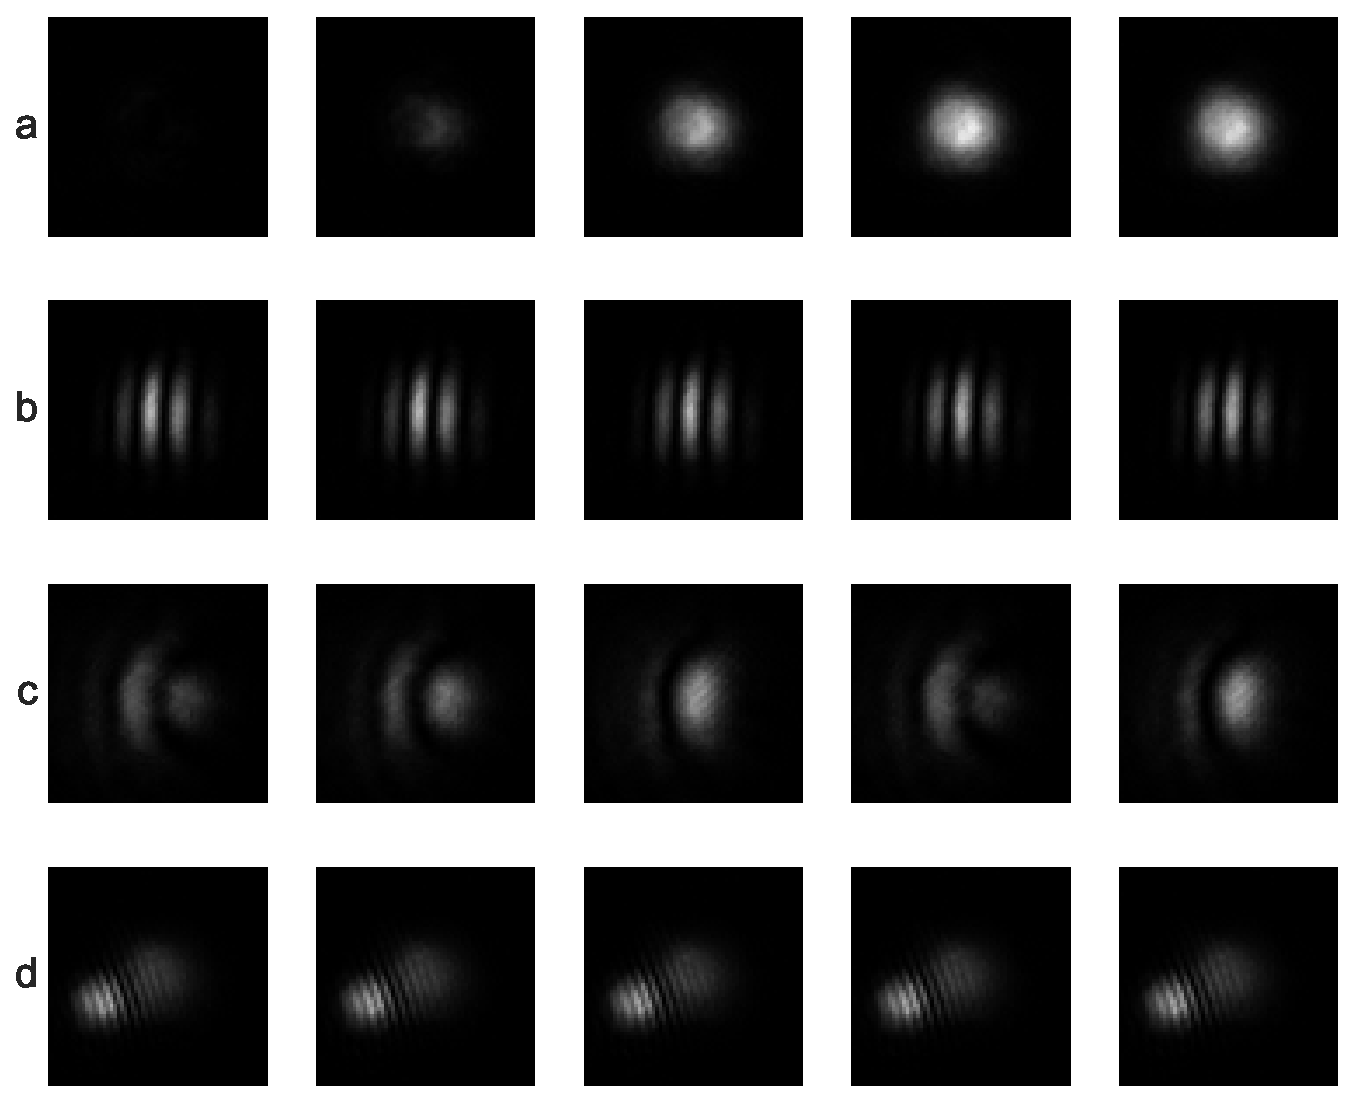
\includegraphics[width=1\linewidth]{images/Env_patterns.pdf}
\column{0.5\linewidth}
\begin{itemize}
    \item[] $V \approx 1$
    \vspace{30pt}
    \item[] $V \approx 0$
    \vspace{30pt}
    \item[] $V \approx 0.1$
    \vspace{30pt}
    \item[] $V \approx 0$
\end{itemize}
\end{columns}
\end{minipage}
    
\end{frame}




\subsection{Метод способный оперировать
действиями различного масштаба и устойчивый к оптическим
шумам}


\begin{frame}{Метод настройки, основанный на алгоритме DQN}
\begin{columns}
\column{0.5\linewidth}
\centering
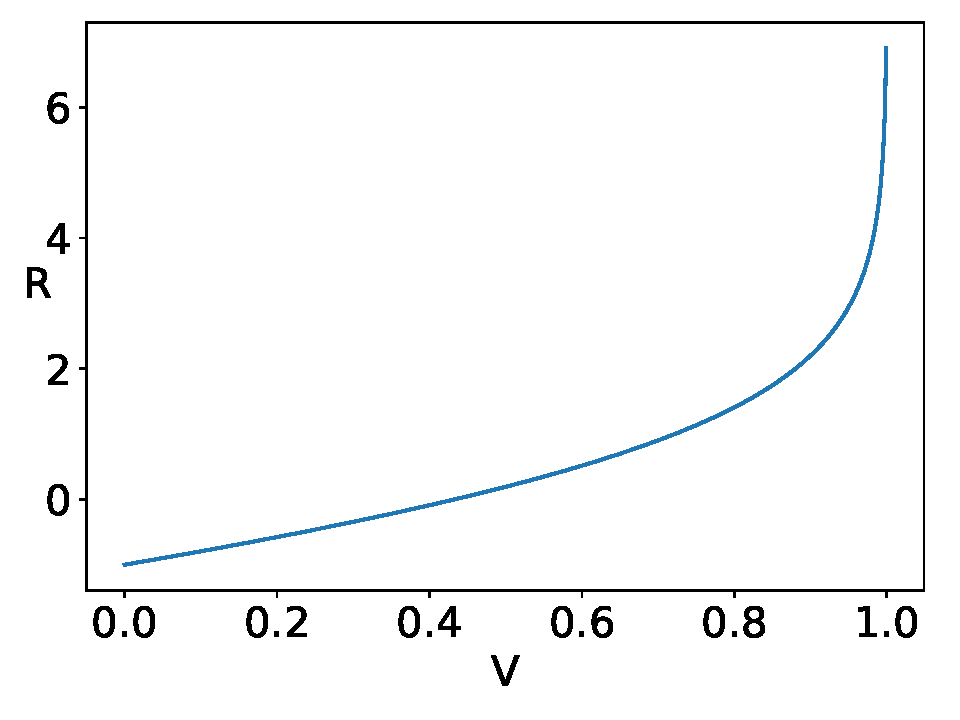
\includegraphics[width=1\linewidth]{images/reward_visib.pdf}
\column{0.5\linewidth}
\textbf{Награда}\\
$R = V - \log(1-V) - 1$\\
$V = 0.95 \to R = 2.9$\\
$V = 0.98 \to R = 3.9$\\
\textbf{Энкодер}\\
3-слойная сверточная  сеть [(32, 8, 4), (64, 4, 2), (64, 3, 1)] (Nature Mnih et.al, 2015)
\end{columns}
\vspace{10pt}
\textbf{Пространство наблюдений} 16 кадров 64x64 пикселя\\
\textbf{Пространство действий} \textcolor{red}{дискретное} (25/31) \\
\textbf{Эпизод} 100 шагов, случайный reset $\pm \alpha_{\mathrm{max}}$, $\pm \Delta_{\mathrm{max}}$\\
\textbf{Параметры} $\gamma = 0.99 \to  \Delta = \frac{1}{1 - \gamma} = \textcolor{red}{100}$, total steps $10^8$, buffer size $10^6$, batch size $32$\\

\end{frame}

\begin{frame}{Метод настройки, основанный на алгоритме TD3}
\begin{columns}
\column{0.5\linewidth}
\centering
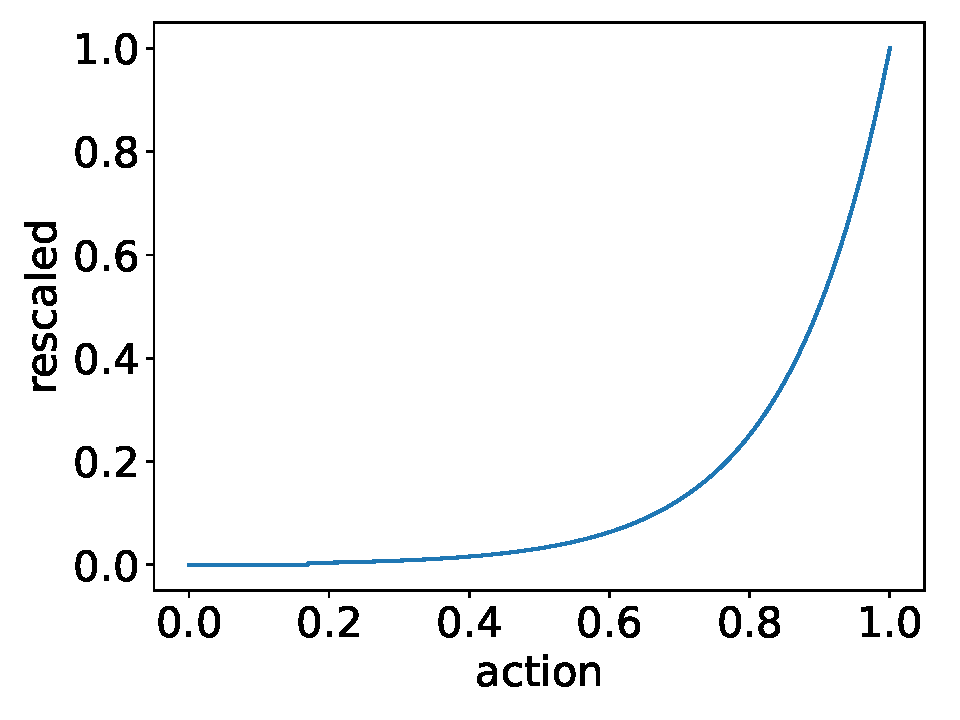
\includegraphics[width=1\linewidth]{images/rescale.pdf}
\column{0.5\linewidth}
\textbf{Награда}\\
$R = V - \log(1-V)$\\
\textbf{Масштабирование действий}\\
\vspace{-15pt}
\begin{equation*}
a^{\prime} =
   \begin{cases}
    {\mathrm{sign}}(a) \cdot 1000^{|a| - 1}, |a| > 0.17
    \\
    0
  \end{cases}
\end{equation*}
\textbf{Энкодер}\\
VGG-16
\end{columns}
\vspace{10pt}
\textbf{Пространство действий} \textcolor{red}{непрерывное} ($\mathcal{R}^4$/$\mathcal{R}^5$)\\
\textbf{Параметры} $\gamma = 0.8 \to  \Delta = \frac{1}{1 - \gamma} = \textcolor{red}{5}$, total steps $10^6$, buffer size $10^5$, batch size $32$ \\

\end{frame}

\begin{frame}{Перенос из симуляции в реальность}
\begin{columns}
\column{0.4\linewidth}
\centering
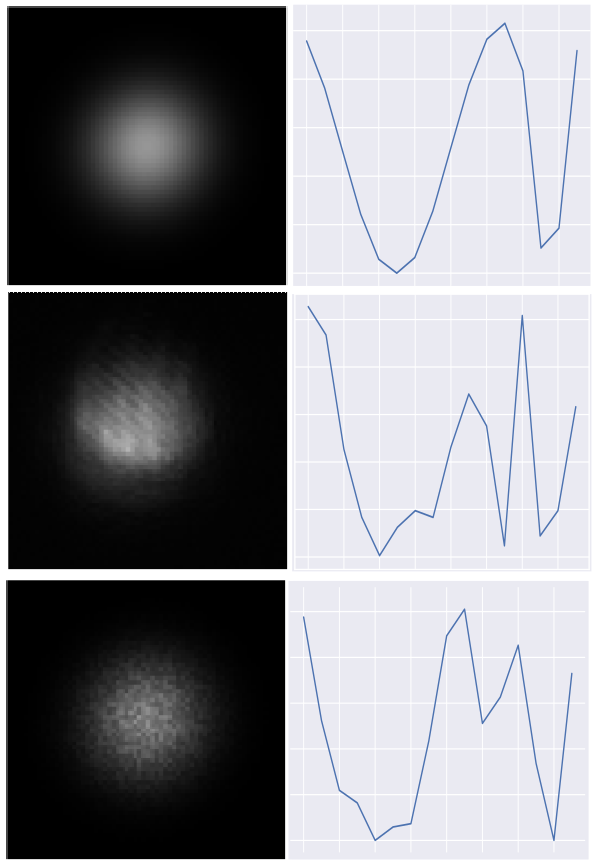
\includegraphics[width=1\linewidth]{beamsamples.png}
\column{0.6\linewidth}
\textbf{в начале каждого эпизода}
\begin{itemize}
    \item radius randomization $\pm 20\%$
\end{itemize}
\textbf{на каждом шаге}
\begin{itemize}
    \item exposure randomization $\pm 30\%$
    \item image noise $20\%$
    \item cycle frame shift
    \item duty cycle randomization
    \item phase noise $\phi \sim \mathcal{N}(\frac{2\pi k}{N}, 0.5)$
\end{itemize}
\end{columns}
\end{frame}

\subsection{Программно-аппаратный комплекс Интерферобот}

\begin{frame}{Программно-аппаратный комплекс Интерферобот}
\begin{columns}
\column{0.35\linewidth}
\centering
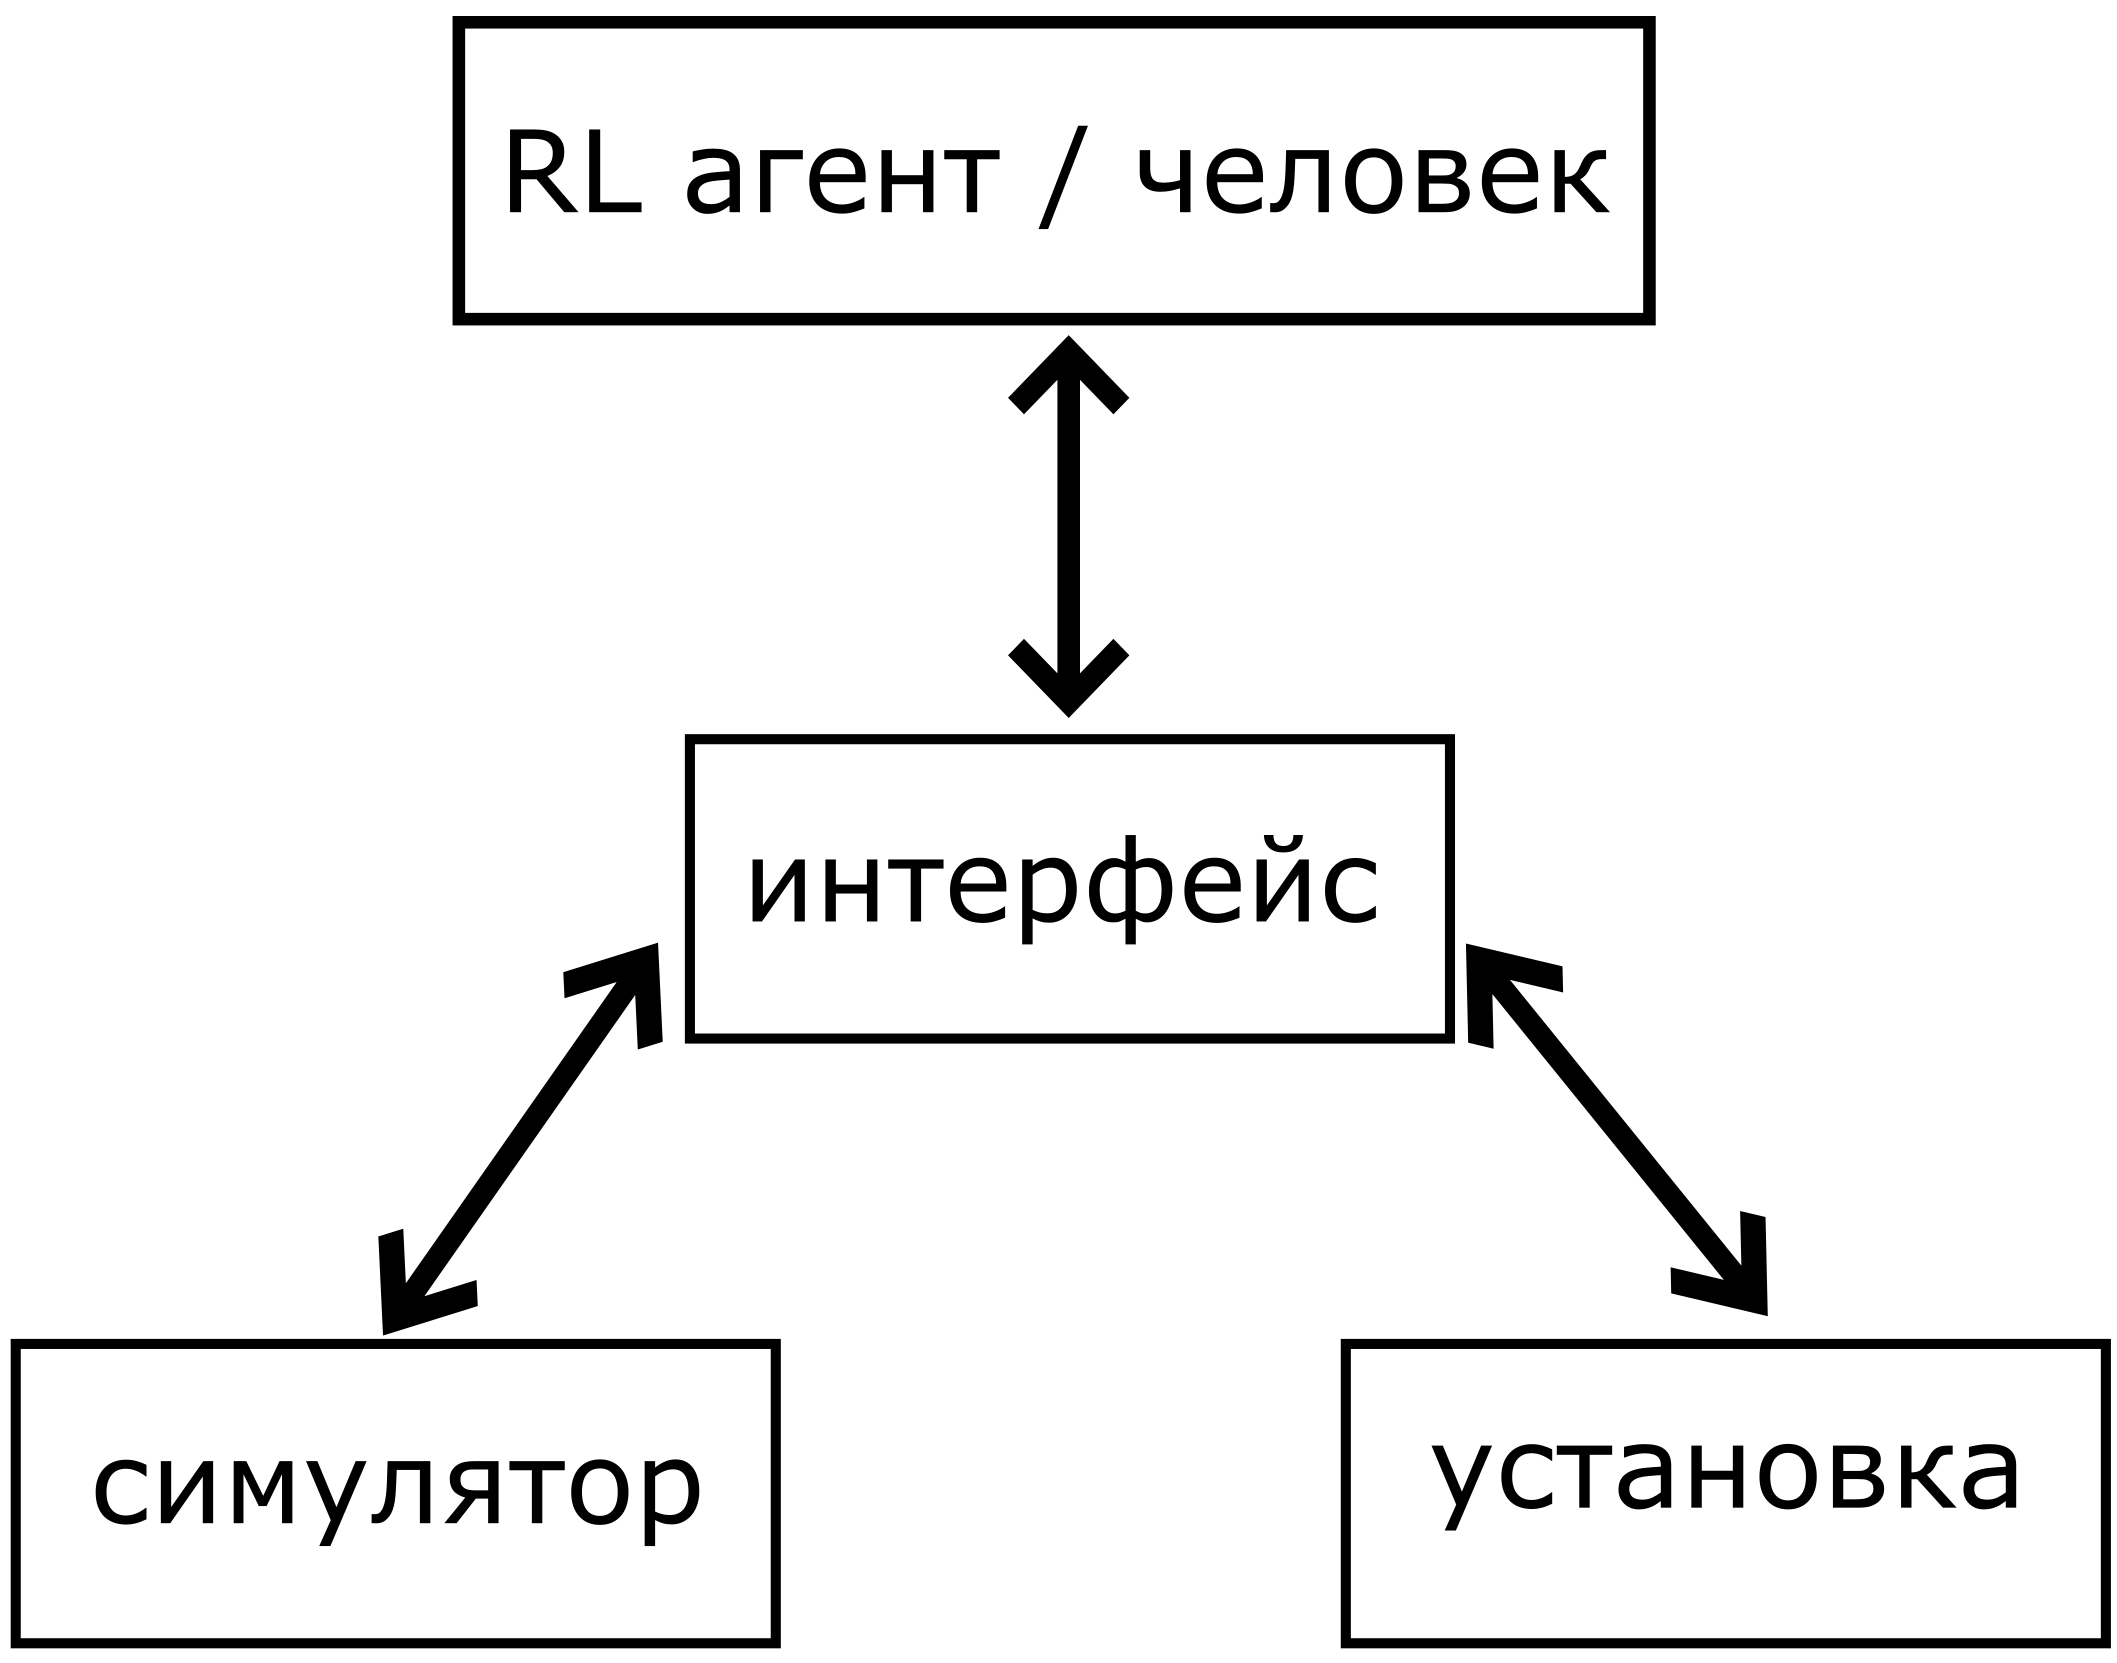
\includegraphics[width=1\linewidth]{images/interferobot_complex.png}
Схема взаимодействия модулей
\column{0.65\linewidth}
\centering
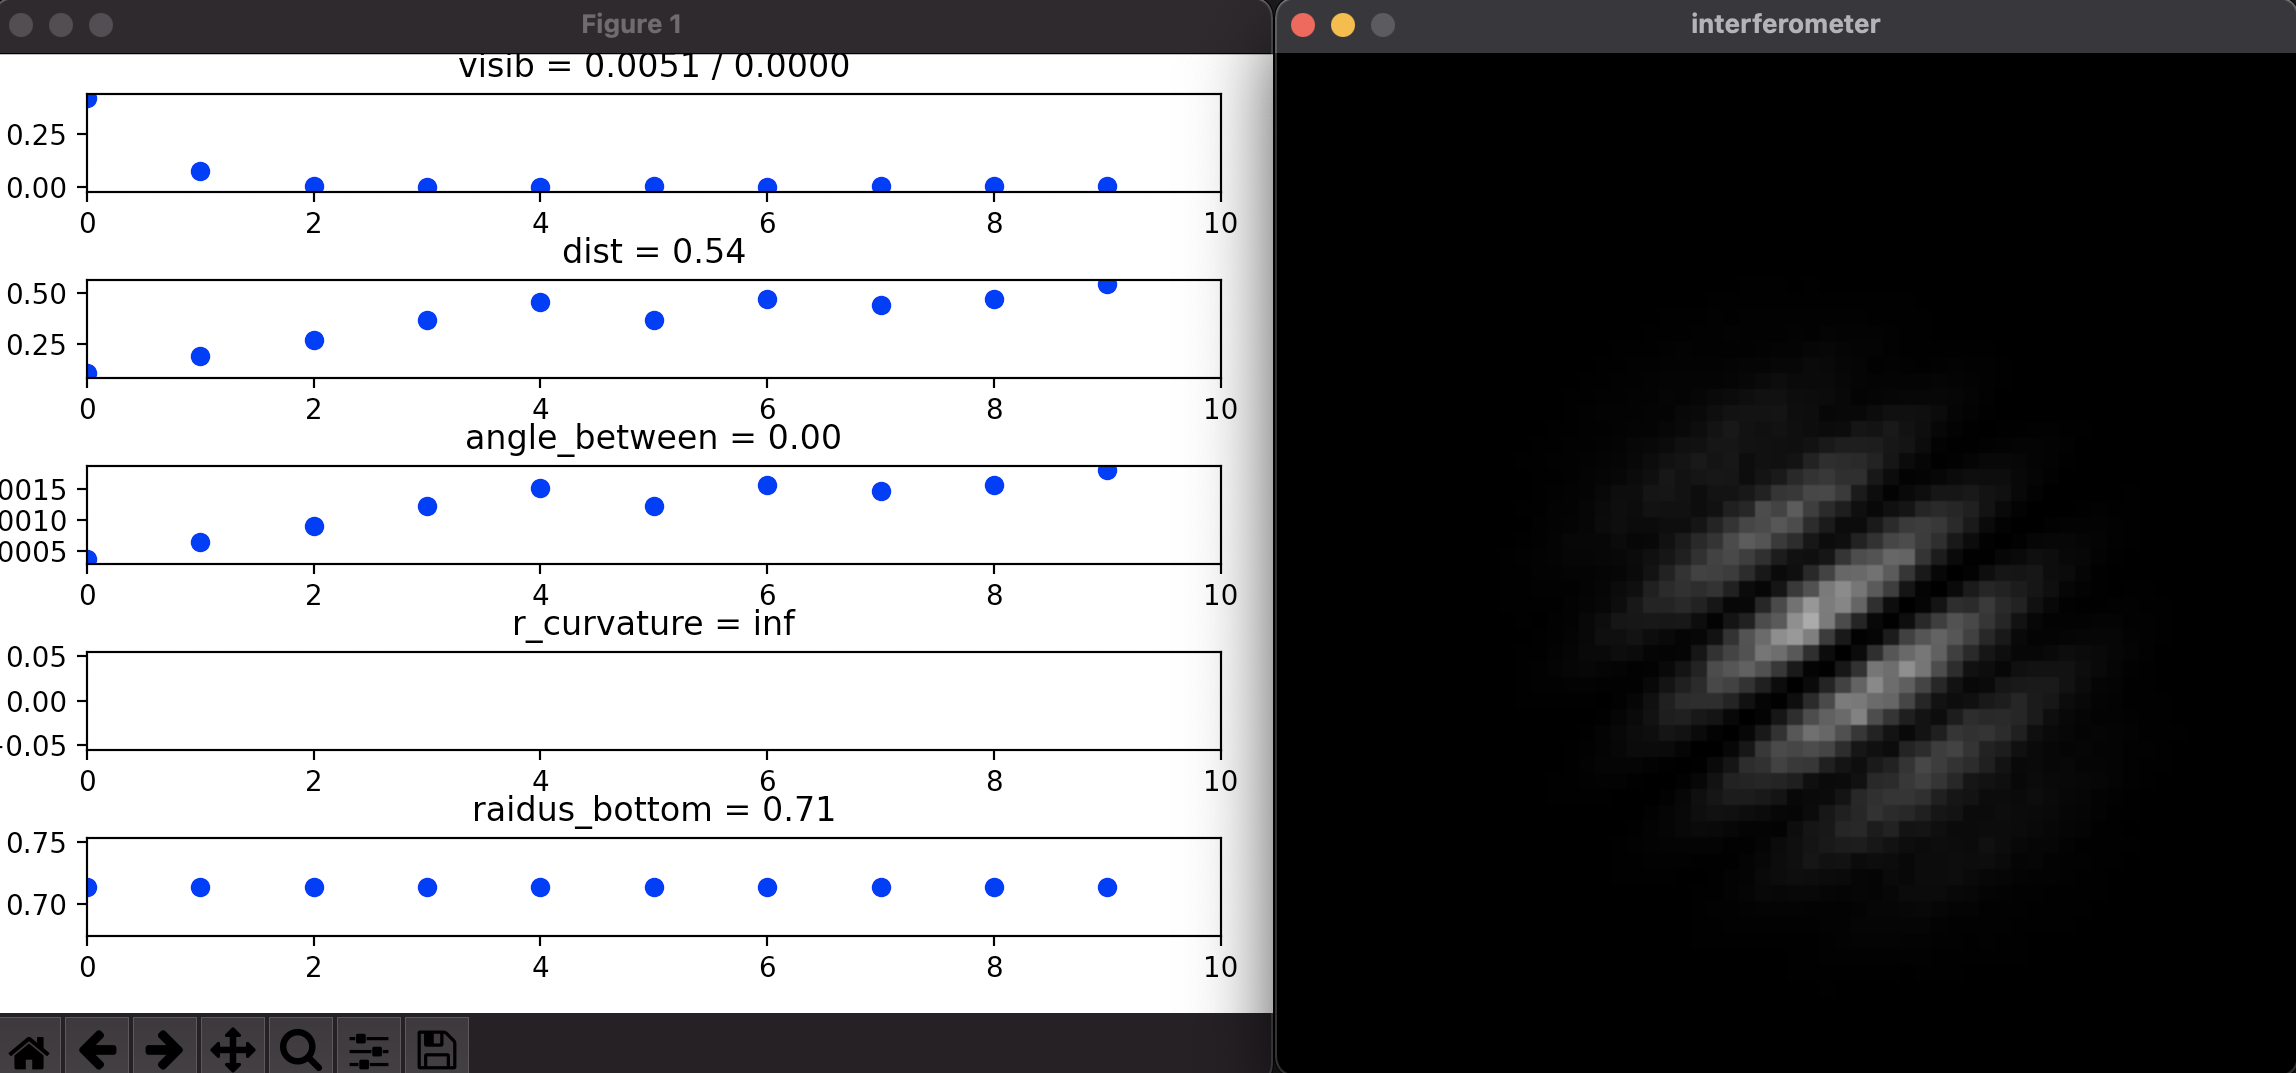
\includegraphics[width=1\linewidth]{images/gui.png}
Графический интерфейс пользователя
\end{columns}
\vspace{15pt}
C++, Python3\\
200 состояний среды (16x64х64) за одну секунду (16 потоков на intel core i7)
\end{frame}

\begin{frame}[allowframebreaks]{Настройка интерферометра Маха-Цендера без линз}
\begin{columns}
\column{0.5\linewidth}
\centering
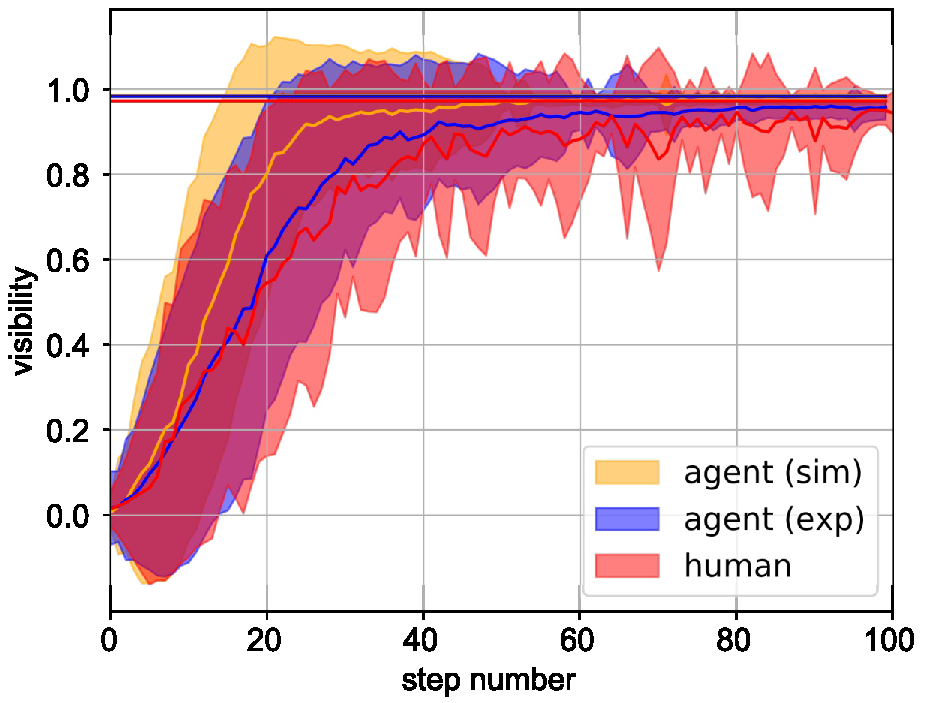
\includegraphics[width=1\linewidth]{images/eval1_visib_step.pdf}
\column{0.5\linewidth}
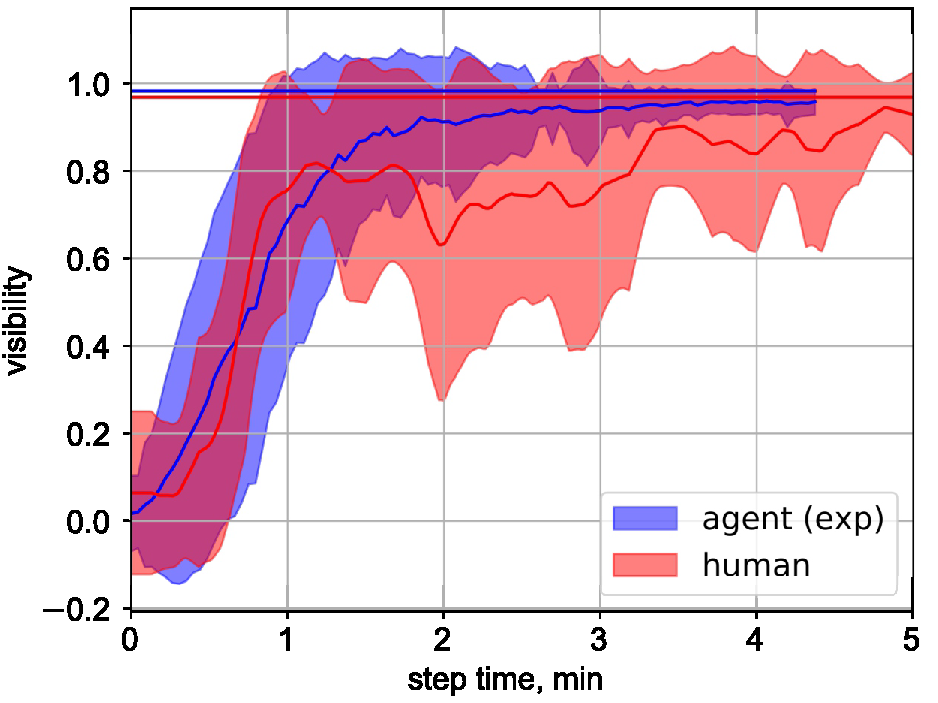
\includegraphics[width=1\linewidth]{images/eval1_visib_time.pdf}
\end{columns}

\vspace{-10pt}

\begin{table} [htbp]
    \centering
    \begin{threeparttable}
        \caption*{Средняя наибольшая видность достигнутая при настройке}
        \begin{tabular}{| p{3cm} || p{3cm} || p{3cm} |}
            \hline
            \hline
            DQN (sim) & DQN (exp) & Human \\
            \hline
            0.986 & 0.983 & 0.972 \\
            \hline
            \hline
        \end{tabular}
    \end{threeparttable}
\end{table}

\centering {\color{orange}Вывод:} дискретный агент работает на уровне опытного специалиста.

\framebreak 

\begin{table} [htbp]
    \centering
    \begin{threeparttable}
        \caption*{{\color{orange} Проверка идеи 1:} Анализ влияния шумов, используемых при обучении агента, на качество настройки физической установки}
        \begin{tabular}{| p{5cm} || p{2cm} || p{2cm} |}
            \hline
            \hline
             & visibility & return \\
            \hline
            All randomizations  & $\textbf{0.96} \pm \textbf{0.02}$ & $\textbf{221} \pm \textbf{54}$ \\
            No radius randomization & $0.74 \pm 0.20$ & $85 \pm 69$ \\
            No exposure randomization& $0.91 \pm 0.04$ & $178 \pm 39$ \\
            No image noise & $0.82 \pm 0.07$ & $129 \pm 43$ \\
            No duty cycle and frame shift  &  $0.89 \pm 0.07$ & $200 \pm 42$ \\
            \hline
            \hline
        \end{tabular}
    \end{threeparttable}
\end{table}
\end{frame}

\begin{frame}[allowframebreaks]{Настройка интерферометра Маха-Цендера с системой линз}
\begin{columns}
\column{0.5\linewidth}
\centering
\includegraphics[width=1\linewidth]{Presentation/images/DQN_vs_TD3.png}
\column{0.5\linewidth}
\centering
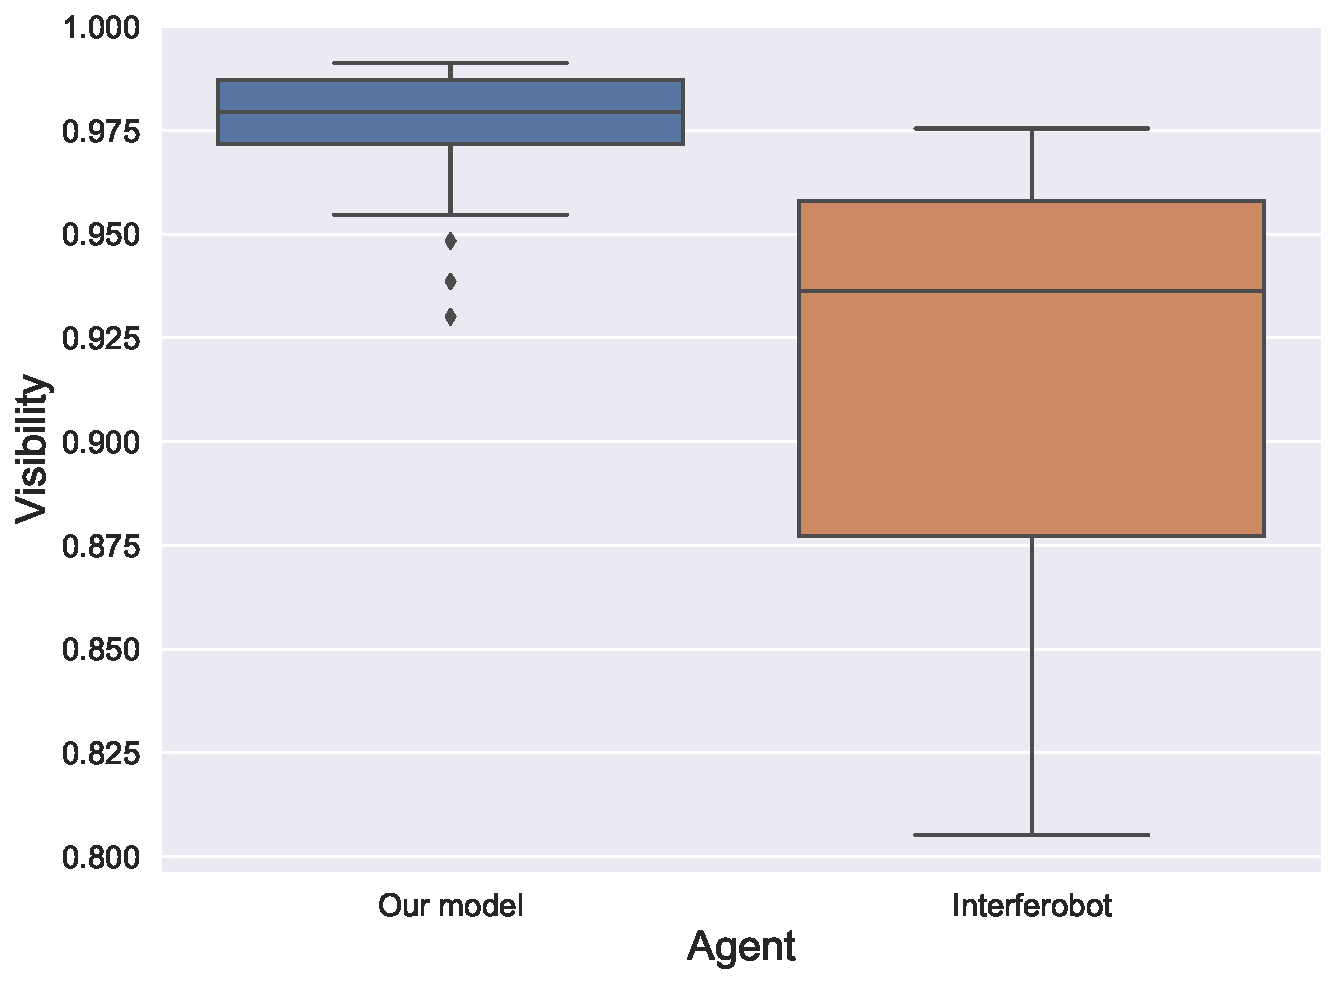
\includegraphics[width=1\linewidth]{images/DQN_vs_TD3_box.pdf}
\end{columns}

\vspace{-10pt}
\begin{table} [htbp]
    \centering
    \begin{threeparttable}
        \begin{tabular}{| p{2cm} || p{2cm} || p{2cm} || p{3cm} |}
            \hline
            \hline
            &V $\ge 0.92$ & V $\ge 0.95$ & V $\ge 0.98$ \\
            \hline
            Human &  93.9 (\textbf{0\%})  & 103.6 (\textbf{0\%}) & 129.6 (10\%)\\
            TD3 &  \textbf{56.16} (\textbf{0\%}) & \textbf{75.06} (\textbf{0\%}) & \textbf{120.1} (\textbf{4\%})\\
            DQN &  98.7 (7.6\%) & 116.1 (7.6\%) & 156.4 (10.6\%)\\
            \hline
            \hline
        \end{tabular}
    \end{threeparttable}
\end{table}

\centering {\color{orange}Вывод:} непрерывный агент работает лучше опытного специалиста.

\framebreak

\begin{table} [htbp]
    \centering
    \begin{threeparttable}
        \caption*{{\color{orange}Проверка идеи 2:} Анализ эффективности фазового шума и масштабирования действий. PN: фазовый шум, AR: масштабирование действий.}
        \begin{tabular}{| p{3cm} || p{3cm} || p{3cm} |}
            \hline
            \hline
            агент & средняя видность за последние 40 шагов & стандартное отклонение \\
            \hline
            TD3 + AR + PN & \textbf{0.98} & \textbf{0.03} \\
            TD3 + AR & 0.95 & 0.06\\
            DQN + PN & 0.90 & 0.08\\
            TD3& 0.83 & 0.18\\
            \hline
            \hline
        \end{tabular}
    \end{threeparttable}
\end{table}

\end{frame}

\begin{frame}{Пример настройки}
\begin{columns}
\column{0.5\linewidth}
    \centering
    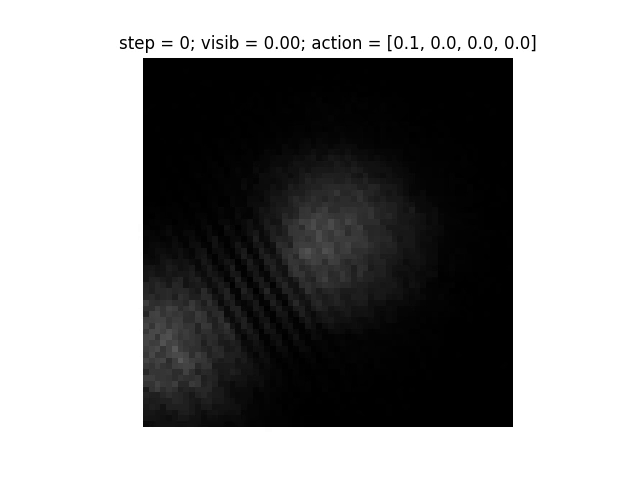
\includegraphics[width=1\linewidth]{Presentation/images/dqn_1.png}
    Дискретный DQN агент
\column{0.5\linewidth}
    \centering
    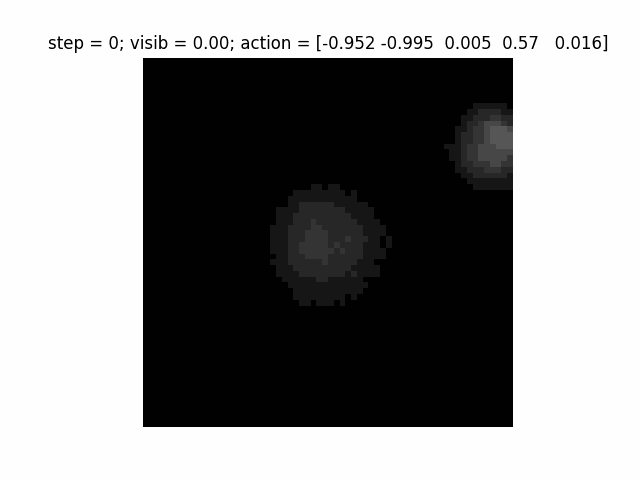
\includegraphics[width=1\linewidth]{Presentation/images/td3_1.png}
    Непрерывный TD3 агент
\end{columns}
\end{frame}


\begin{frame}{Выводы}
\begin{itemize}
    \item[\textcolor{ForestGreen}{\checkmark}] Разработаны алгоритмы, подбора параметров симуляции и масштабирования пространства действий. 
    \item[\textcolor{ForestGreen}{\checkmark}] На основе предложенных алгоритмов реализованы методы настройки оптического интерферометра основанные на обучении с подкреплением.
    \begin{itemize}
        \item[--] Разработан симулятор интерферометра Маха-Цендера.
        \item[--] Разработан программно-аппаратный комплекс Интерферобот.
        \item[--] Предложен набор шумов и функция награды.
        \item[--] Качество настройки с использованием разработанного метода превосходит качество настройки эксперта.
    \end{itemize}
    
    
\end{itemize}
    



\end{frame}

% \subsection{Не нумерованные}


\section{Глава 3. Метод управления линейной и угловой скоростью шагающего робота основанный на обучении с подкреплением}

\begin{frame}
    \frametitle{Структура диссертационной работы}
    \begin{itemize}
        \item \underline{Глава 1.} Обзор методов обучения с подкреплением и их применения в роботике. 
        \item \underline{Глава 2.} Разработка метода, способного оперировать действиями различного масштаба, устойчивого к шумам, и его применение для настройки оптического интерферометра (вызов 1,2).
        {\color{orange}\item \underline{Глава 3.} Метод, который позволяет достичь сходимости к хорошему оптимуму для многозадачного агента и его применение  для управления движением шагающего робота (вызов 3).}
        \item \underline{Глава 4.} Иерархический алгоритм, комбинирующий алгоритмический и нейросетевой подходы и его применение для управления агентом в среде NetHack (вызов 4).
    \end{itemize}
\end{frame}

\begin{frame}{Постановка задачи оптимизации}

$$V(s_t) = \max_{a \in \mathcal{A}}\ex_{r_{t+1},s_{t+1}}\left[r_{t+1} + \gamma V(s_{t+1})\right]$$
$$\pi(s_t) = \argmax_{a \in \mathcal{A}}\ex_{r_{t+1},s_{t+1}}\left[r_{t+1} + \gamma V(s_{t+1})\right]$$

Особенности:
\begin{enumerate}
    \item Многозадачность - хотим решать несколько задач с помощью единого агента.
    \item Сложная функция награды - сходимость к суб-оптимальной стратегии. 
    \item Высокая размерность пространства состояний $s \in \mathcal{R}^N$.
\end{enumerate}
\end{frame}

\begin{frame}{Алгоритм: обучение по расписанию для многозадачного агента}

\begin{minipage}{\linewidth}

\begin{columns}
\column{0.5\linewidth}
\begin{enumerate}
    \item Для многозадачности будем рассматривать каждую задачу как часть состояния агента $s = (o, t)$, $t$ - текущая задача. 
    \item Будем увеличивать штрафные коэффициенты в функции награды линейно по мере обучения агента:
    \vspace{-10pt}
    \begin{equation*}
        r = r_{task} - \frac{n}{N} \cdot \sum_i r_{\mathrm{penalty}_i}
    \end{equation*}
\end{enumerate}

\column{0.5\linewidth}
\begin{algorithm}[H]
\KwData{
распределение задач $T$
}
\KwResult{параметры агента $\theta$} 
\While{n < $N$}{
  выбираем задачи $t_i \sim T$\;
  \ForEach {$t_i$} {
    генерируем траекторию $\tau \sim \pi_{\theta}(\cdot |t_i)$\;
  }
  обновляем параметры
  $\theta \gets \theta - \alpha \nabla \mathcal{L}(\theta)$\;
}
\end{algorithm}
\end{columns}
\end{minipage}
\begin{minipage}{\linewidth}

\vspace{5pt}
\setcounter{footnote}{0} 
Связанные работы (нет многозадачности)\footnote[frame]{Hwangbo, J. et al., Learning agile and dynamic motor skills for legged robots, Science Robotics, 2019.}\footnote[frame]{Lee, J. et al. Learning quadrupedal locomotion over challenging terrain, Science Robotics, 2020.}
\end{minipage}

    
\end{frame}

\begin{frame}{Практическая задача: управление шагающим роботом}
\begin{columns}
\column{0.5\linewidth}
\centering
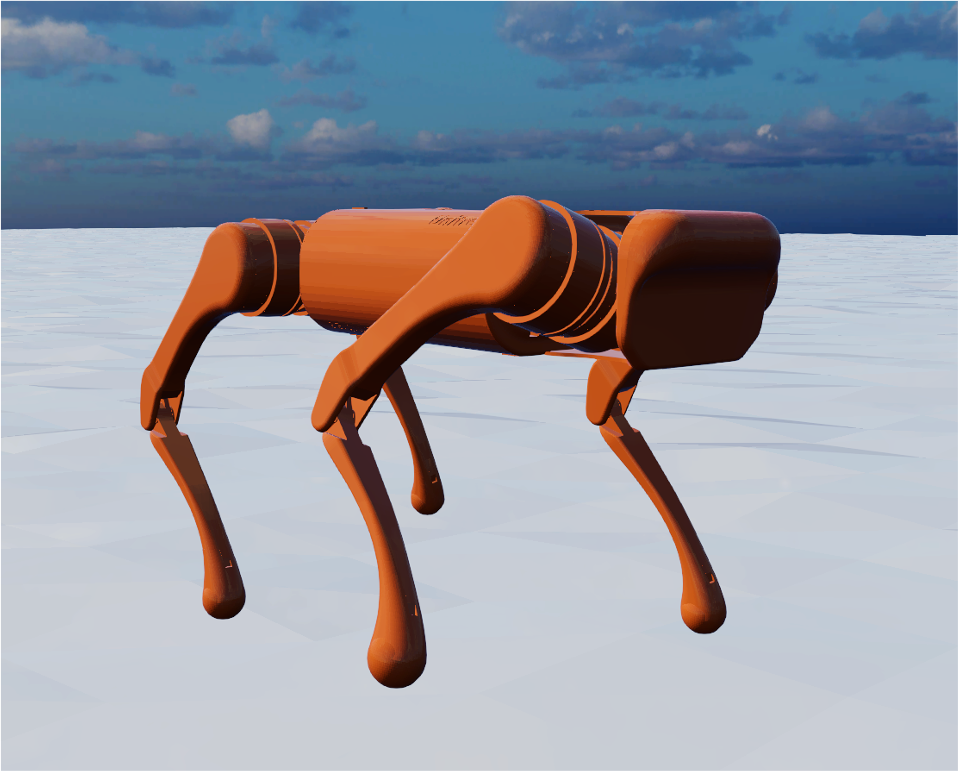
\includegraphics[width=1\linewidth]{unitree_a1.png}
\column{0.5\linewidth}
\begin{itemize}
    \item ``Движение вперед / назад''
	\item ``Движение вперед с заданной скоростью''
    \item ``Поворот по / против часовой стрелке''
\end{itemize}
\end{columns}
\textbf{Пространство наблюдений} положение корпуса, суставов, линейные и угловые скорости ($\mathcal{R}^{50}$) 
\\
\textbf{Пространство действий} целевые положения суставов ($\mathcal{R}^{12}$ )

\end{frame}

\begin{frame}{Метод обучения стратегии для управления движением
шагающего робота с заданной линейной и угловой скоростью}
\begin{multline*}
    r = k_{torso\ height} \cdot r_{torso\ height} +
    k_{torque} \cdot r_{torque} +\\
    k_{joint\ speed} \cdot r_{joint\ speed} +
    k_{slip} \cdot r_{slip} +\\
    k_{work} \cdot r_{work} + 
    k_{ground\ impact} \cdot r_{ground\ impact} +\\
    k_{z\ acceleration} \cdot r_{z\ acceleration} +  k_{velocity} \cdot r_{velocity} +\\
    k_{transverse\ and\ rotation} \cdot r_{transverse\ and\ rotation}
\label{eq:unitree_reward}
\end{multline*}

\begin{align*}
& r_{velocity} = \mathrm{clip}(V_x \cdot D / \hat{V_x}, 0, 1) \hspace{18pt}\text{``Движение вперед / назад''}\\
& r_{velocity} = \max(1 - |V_x / \hat{V_x} - 1|, 0) \hspace{1pt}\text{``Движение вперед с заданной скоростью''}\\
& r_{velocity} = \mathrm{clip}(W_z \cdot D / \hat{W_z}, 0, 1) \hspace{13pt}\text{``Поворот по / против часовой стрелки''}
\end{align*}
\end{frame}

\begin{frame}{Оценка результатов работы в симуляции}
\begin{figure}[h]
\begin{subfigure}{.5\textwidth}
  \centering
  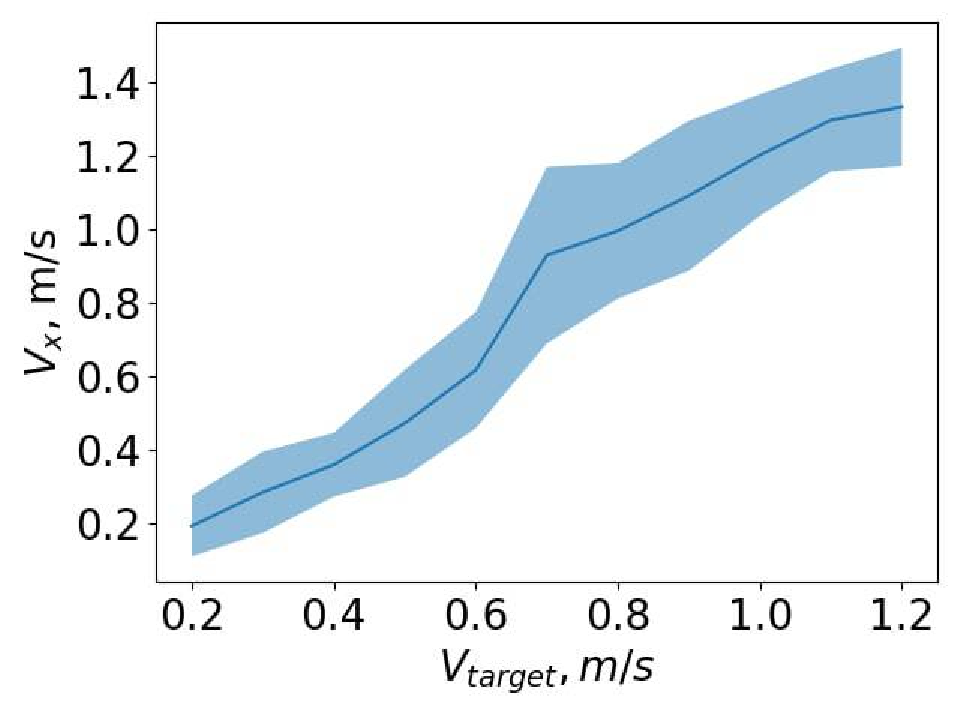
\includegraphics[width=1\textwidth]{images/vx}
\end{subfigure}%
\begin{subfigure}{.5\textwidth}
  \centering
  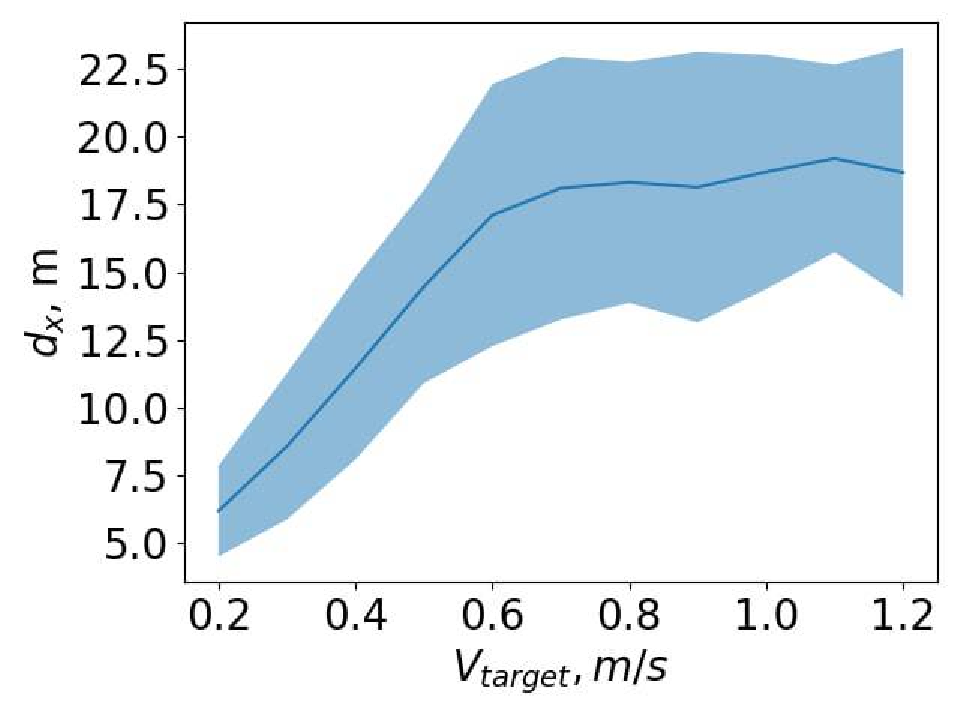
\includegraphics[width=1\textwidth]{images/dx}
\end{subfigure}%
\end{figure}
\begin{table} [htbp]
    \centering
    \begin{threeparttable}
        \begin{tabular}{| p{1cm} || p{2cm} | p{2cm} | p{2cm} |p{2cm} |}
            \hline
            \hline
            Задача & Вперед & Назад & По часовой & Против часовой \\
            \hline
            $R_{total}$ &	529 $\pm$ 124 &	508 $\pm$ 98 &	85 $\pm$ 219 &	165 $\pm$ 155 \\
            $N_{steps}$ & 3263 $\pm$ 633 &	3136 $\pm$ 545 &	2057 $\pm$ 1208 &	2095 $\pm$ 1325 \\
            \hline
            \hline
        \end{tabular}
    \end{threeparttable}
\end{table}
\end{frame}

\begin{frame}{Выводы}
\begin{itemize}
    \item[\textcolor{ForestGreen}{\checkmark}] Был разработан метод обучения робота Unitree A1 решать различные задачи перемещения.
    \item[\textcolor{ForestGreen}{\checkmark}] Разработанная функция награды побуждает агента следовать плавной и безопасной стратегии.
\end{itemize}
\end{frame}



\section{Глава 4. Иерархический алгоритм, комбинирующий алгоритмический и
нейросетевой подходы и его применение для управления агентом в среде NetHack}


\begin{frame}
    \frametitle{Структура диссертационной работы}
    \begin{itemize}
        \item \underline{Глава 1.} Обзор методов обучения с подкреплением и их применения в роботике. 
        \item \underline{Глава 2.} Разработка метода, способного оперировать действиями различного масштаба, устойчивого к шумам, и его применение для настройки оптического интерферометра (вызов 1,2).
        \item \underline{Глава 3.} Метод, который позволяет достичь сходимости к хорошему оптимуму для многозадачного агента и его применение  для управления движением шагающего робота (вызов 3).
        {\color{orange}\item \underline{Глава 4.} Иерархический алгоритм, комбинирующий алгоритмический и нейросетевой подходы и его применение для управления агентом в среде NetHack (вызов 4).}
    \end{itemize}
\end{frame}

\begin{frame}{Постановка задачи оптимизации}

$$V(s_t) = \max_{a \in \mathcal{A}}\ex_{r_{t+1},s_{t+1}}\left[r_{t+1} + \gamma V(s_{t+1})\right]$$
$$\pi(s_t) = \argmax_{a \in \mathcal{A}}\ex_{r_{t+1},s_{t+1}}\left[r_{t+1} + \gamma V(s_{t+1})\right]$$

Особенности:
\begin{enumerate}
    \item Процедурная генерация среды.
    \item Разреженная функция награды $|s| \ll |\mathcal{S}|: r(s,a,s') \neq 0$.
    \item Необходимость следования различным стратегиям в зависимости от текущего состояния. 
    \item Многомодальные наблюдения $s = (s_{\mathrm{text}}, s_{\mathrm{img}}, s_{\mathrm{num}})$.
\end{enumerate}
\end{frame}

\setcounter{footnote}{0} 
\begin{frame}{Алгоритм: объединение обучаемых и алгоритмических стратегий в иерархического агента\footnotemark\footnotemark}

\begin{minipage}{\linewidth}
\begin{columns}
\column{0.5\linewidth}
\begin{enumerate}
    \item Декомпозиция на отдельные стратегии может существенно помочь в задачах, где нужно уметь переключаться между различными навыками.
    \item Переключение между обучаемыми и алгоритмическими стратегиями происходит в зависимости от состояния среды. 
\end{enumerate}

\column{0.5\linewidth}
\begin{algorithm}[H]
\SetKwComment{Comment}{/* }{ */}
\SetKw{Continue}{continue}
\KwData{condition, $\pi_{\theta}$, $<\pi_{\mathrm{alg}}>$}
s $\gets$ env.reset()\;
\While{not done}{
  \eIf{condition(s)}{
    $a \sim \pi_{\theta}(s)$\;
  }{
    $\pi = \mathrm{rank}(\pi_{\mathrm{alg}}, s)$
    $a \sim \pi(s)$
  }
  s, r, done, info = env.step(a)\;
}
\end{algorithm}
\end{columns}
\end{minipage}

\begin{minipage}{\linewidth}

%\footnote[frame]{Sutton, R., et.all. Between MDPs and semi-MDPs: A framework for temporal abstraction in reinforcement learning. Artificial Intelligence (1999)}
\end{minipage}
\footnotetext[1]{Barreto, A., et al., The Option Keyboard: Combining Skills in Reinforcement Learning, NeurIPS, 2019.}
\footnotetext[2]{Gao, J., et al., Deep Reinforcement Learning for Indoor Mobile Robot Path Planning, Sensors (Basel), 2020.}
    
\end{frame}

\begin{frame}
\frametitle{Задача: NetHack challenge}
\begin{columns}
\column{0.6\linewidth}
  \centering
  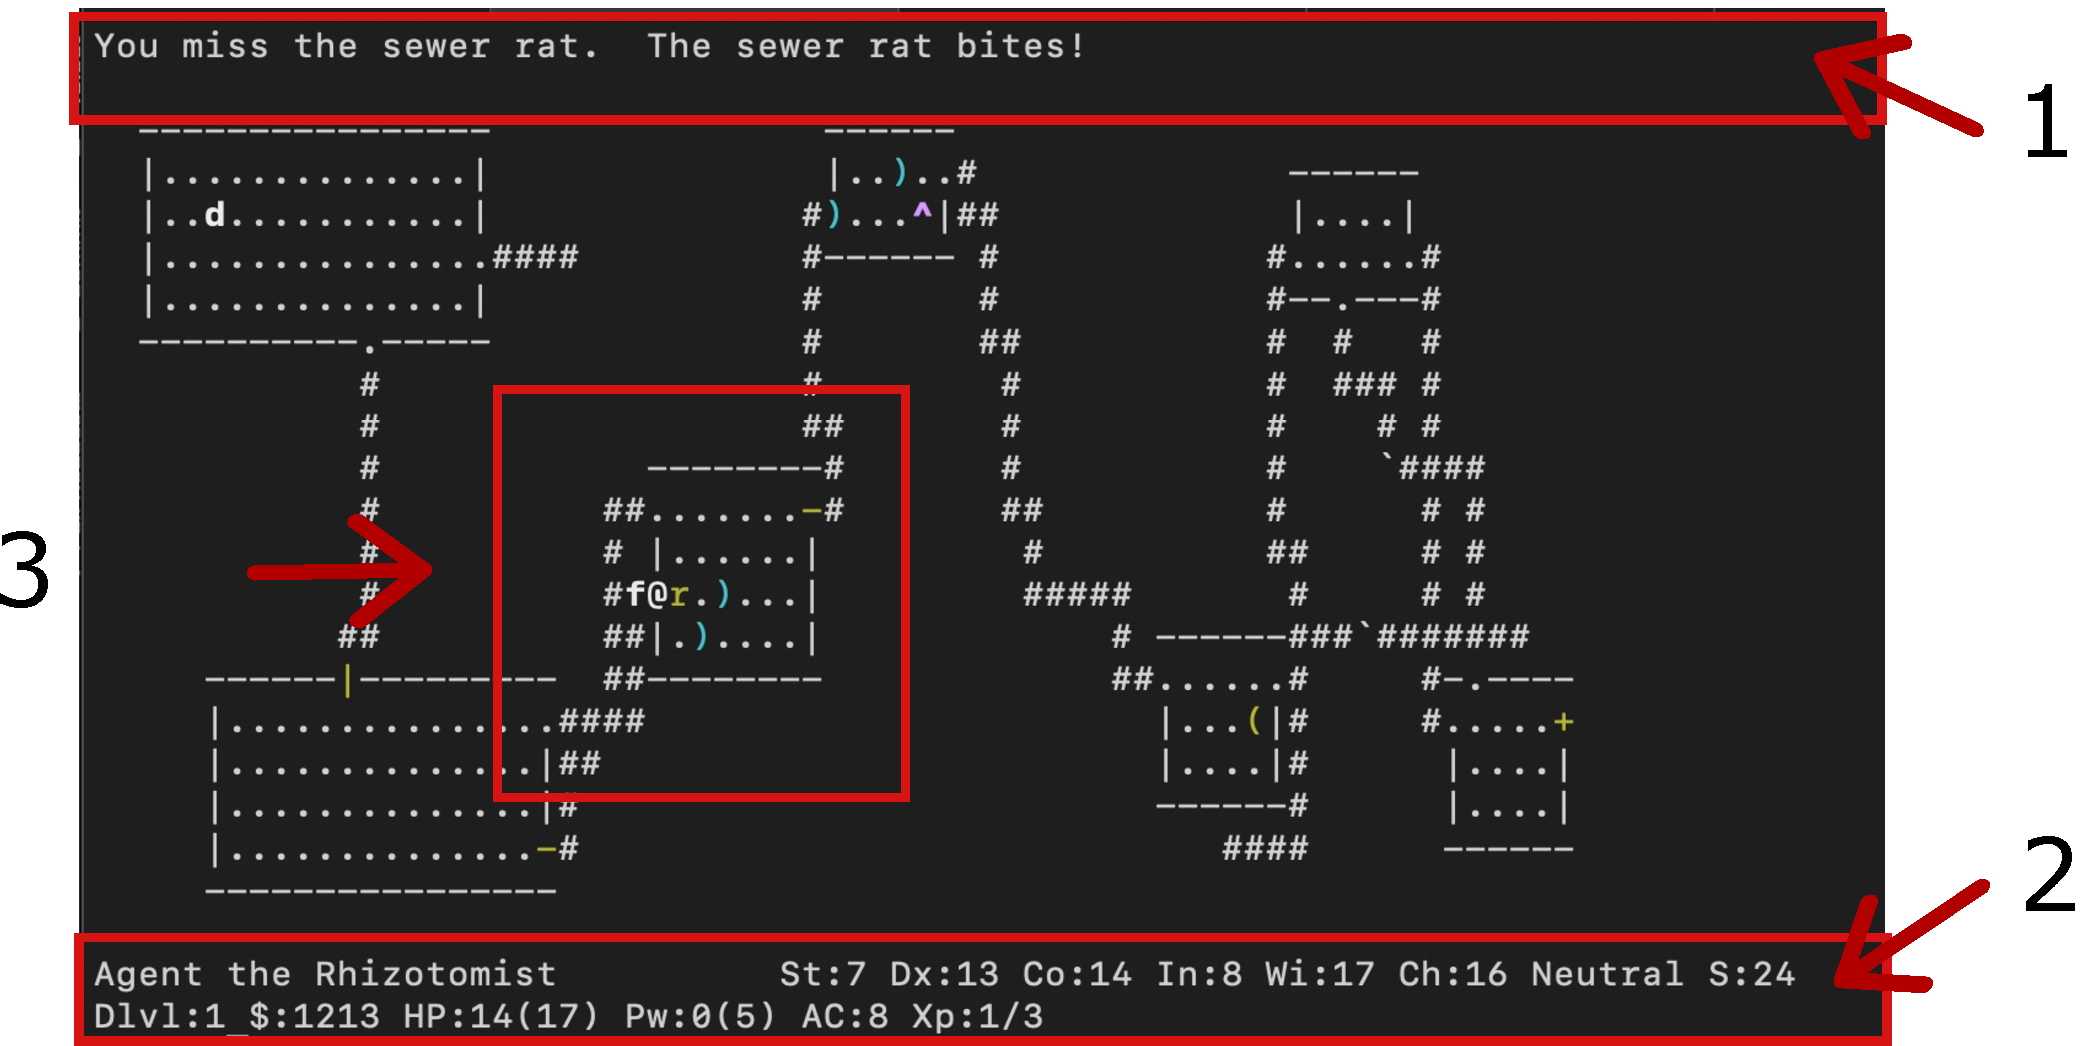
\includegraphics[width=1\linewidth]{images/nethack_map_view.pdf}
\column{0.55\linewidth}
\begin{enumerate}
    \item текстовое сообщение описывающее текущее событие
    \item статистика агента (здоровье, золото, сила, и др.) 
    \item окно центрированное возле текущего положения агента (@).
\end{enumerate}
\end{columns} 
\vspace{20pt}
В чем ``challange''?
\begin{itemize}
    \item Процедурная генерация среды
    \item NetHack – очень длинная игра
    \item Много модальные наблюдения
    \item Сложное пространство действий
\end{itemize}


\end{frame}

\subsection{Декомпозиция игры NetHack на подзадачи}

\begin{frame}{Декомпозиция игры NetHack на подзадачи}
\begin{columns}
\column{0.5\linewidth}
\centering
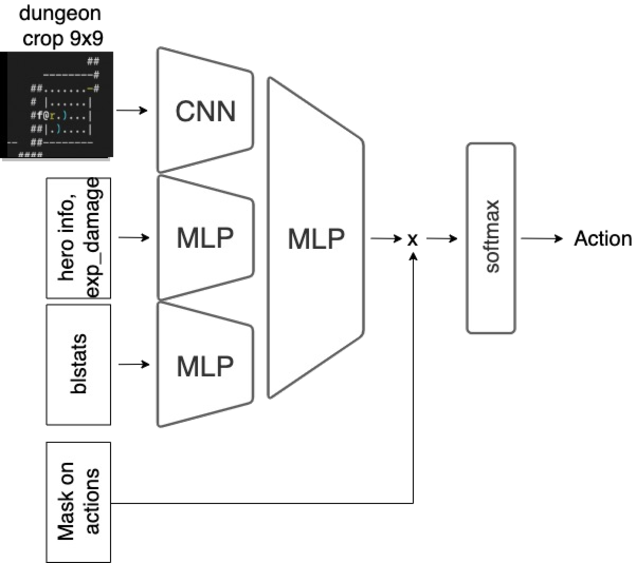
\includegraphics[width=1\linewidth]{images/raph_arch.pdf}
\column{0.5\linewidth}
\textbf{Пространство действий}. 
\begin{itemize}
    \item шаг или ближняя атака (x8 направлений)
    \item дальняя атака (x8 направлений)
    \item пропуск хода
    \item заклинание Elbereth
    \item молитва
\end{itemize}
\textbf{Передача управления}. 
$distance(agent, monster) < 5$
\end{columns}
\end{frame}

\subsection{Объединение RL и алгоритмического подхода}

\begin{frame}
\frametitle{Обучение иерархического агента совмещающего обучение с подкреплением и алгоритмический подход}
\begin{columns}
\column{0.7\linewidth}
\centering
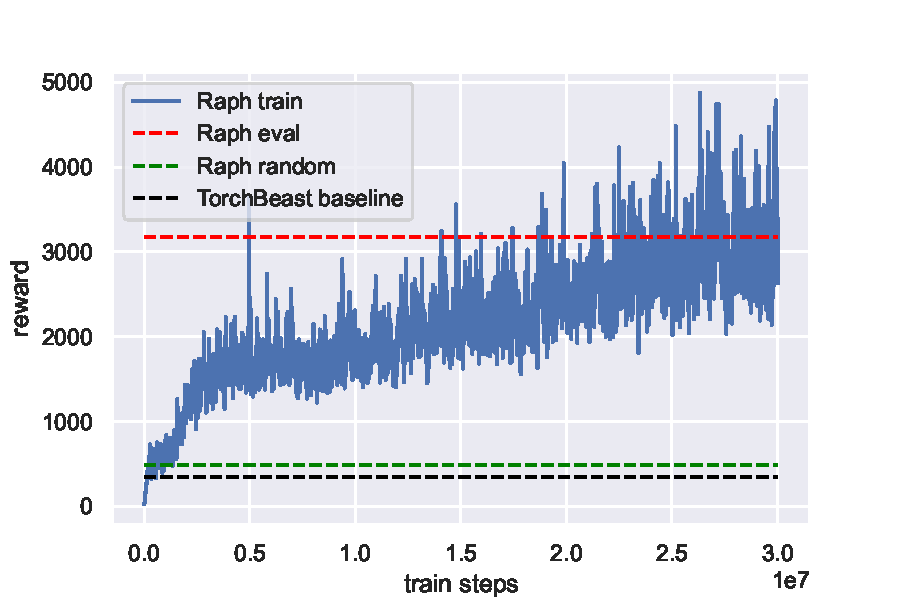
\includegraphics[width=1\linewidth]{images/raph_train.pdf}
\column{0.5\linewidth}
\begin{itemize}
    \item ближняя атака 66\%
    \item дальняя атака 21.6\%
    \item пропуск хода 11\%
    \item ``Elbereth'' 0.3\%
    \item молитва 0.1\%
\end{itemize}
\end{columns}
\end{frame}


\begin{frame}{Выводы}
\begin{itemize}
    \item[\textcolor{ForestGreen}{\checkmark}] Предложен метод объединения обучаемого и алгоритмического подходов в рамках одного агента. С использованием предложенного метода реализован гибридный нейро-символьный агент для среды NetHack.
    \item[\textcolor{ForestGreen}{\checkmark}] В реализованном методе RL агент решает одну из наиболее сложных задач возникающих в среде NetHack — сражение с монстрами.
    \item[\textcolor{ForestGreen}{\checkmark}] В соревновании по игре NetHack (NeurIPS 2021 Competition Track) агент занял \textcolor{orange}{первое место} среди 37 команд из 19 стран мира.
\end{itemize}
    
\end{frame}

%\begin{frame}
%    \frametitle{Изображения по-вертикали}
%    \centering
%    \vfill
%    \includegraphics[width=0.8\linewidth,height=0.1\textheight]{latex%} \\
%    \TeX
%    \vfill
%    \includegraphics[width=0.8\linewidth,height=0.2\textheight]{latex%} \\
%    \LaTeX
%    \vfill
%    \includegraphics[scale=0.2]{latex} \\
%    \vfill
%\end{frame}


%\begin{frame}
%    \frametitle{Изображения по-горизонтали}
%    \begin{minipage}[t]{0.47\linewidth}
%        \textbf{Составная \\ подпись 1}
%        \center{\includegraphics[width=1\linewidth]{knuth1}}
%    \end{minipage}
%    \hfill
%    \begin{minipage}[t]{0.47\linewidth}
%        \textbf{Составная \\ подпись 2}
%        \center{\includegraphics[width=1\linewidth]{knuth2}}
%    \end{minipage}
%\end{frame}


%\begin{frame}
%    \frametitle{Разделяющие линии}
%    \begin{minipage}[c]{0.47\linewidth}
%        \center{\includegraphics[width=1\linewidth]{latex}}
%        \bigskip
%        \hrule{}
%        \bigskip
%        \textbf{Составная \\ подпись 1}
%    \end{minipage}
%    \hfill
%    \vrule{}
%    \hfill
%    \begin{minipage}[c]{0.47\linewidth}
%        \flushright
%        \textbf{Составная \\ подпись 2}
%        \center{\includegraphics[width=1\linewidth]{knuth2}}
%    \end{minipage}
%\end{frame}

%\begin{frame}
%    \frametitle{Четыре изображения}
%    \centering
%    \includegraphics[width=0.35\linewidth,angle=35]{latex}
%    \includegraphics[width=0.35\linewidth,angle=135]{latex}\\
%    \includegraphics[width=0.35\linewidth,angle=15]{latex}
%    \includegraphics[width=0.35\linewidth,angle=-15]{latex}
%\end{frame}

